\section{Introduction}
\label{sec:introduction}

Many world action models (WAMs) produce predicted futures alongside robot actions \citep{kim2026cosmospolicy,nvidia2026cosmos3}. Joint generation, however, does not imply that action computation uses the predicted future: a policy could map the current observation and instruction directly to an action while producing a plausible future as an auxiliary output. Alternatively, predicted-future representations may serve as a computational workspace, encode a prospective robot pose for inverse dynamics \citep{hu2025vpp,du2023unipi}, or represent consequences used to evaluate actions \citep{ebert2018visualforesight,du2024videolanguage}.

RIFT provides the closest prior causal evidence by masking reads from and editing values at predicted-future positions in several WAMs \citep{zhang2026rift}. These interventions establish that behavior depends on information carried through the predicted-future interface. Because disrupting the interface can move an action in any direction, however, they do not reveal how a particular coherent future shapes behavior. We adapt mechanistic interventions to this joint video--action modality to make directional, testable claims about both future content and its computational pathway.

We ask three questions: Does a native future representation direct action; does this effect recur across inference organizations; and which internal pathway carries it? In Stage 1, we insert one rollout's future representation into another rollout from the same state. The receiving rollout is the \emph{recipient}; the source is the \emph{donor}. We recompute the recipient action while fixing the present and recipient action randomness. The donor action is withheld and used only as a directional reference. In Stage 2, we cross the visible future and future-token attention K/V sources in Cosmos 3, separating what is shown from what action queries read.

The experiments yield three findings. First, an outcome-unfiltered four-source Cosmos 3 evaluation recovers the installed source from the recomputed action in all 1,080 off-diagonal comparisons across 90 states; FastWAM, DreamZero, and LingBot-VA replicate source-specific control across joint and ordered video-first inference. Second, Cosmos Policy's effect survives simulator execution and is concentrated in visual future targets, especially the wrist camera, whereas isolated robot or object pixels cannot reproduce Cosmos 3's complete-video effect. Third, Cosmos 3 actions follow the future-token K/V source in all 42 crossed comparisons. Together, these results show reproducible counterfactual control by native future representations and identify a major internal route for that control.

\paragraph{Related work.}
Visual robot policies may infer actions from predicted video, condition on its representation, or generate futures and controls jointly \citep{du2023unipi,hu2025vpp,guo2024pad,li2025uva,kim2026cosmospolicy,nvidia2026cosmos3,ye2026dreamzero,li2026cauva}. These objectives do not establish how a particular future participates in inference. Recent work tests whether explicit rollout is needed \citep{li2025uva,yuan2026fastwam}, aligns foresight and action representations \citep{qiu2026agra}, or intervenes on predicted-future positions \citep{zhang2026rift}. Activation and path patching test whether a representation or route affects output \citep{vig2020causalmediation,meng2022rome,goldowskydill2023pathpatching}. We use within-state counterfactuals and directional source identification to determine what future representations control and to trace one route through predicted-future K/V \citep{zhang2024activationpatching}.

\section{Two-Stage Intervention Design}
\label{sec:methods}

\begin{figure*}[t]
  \centering
  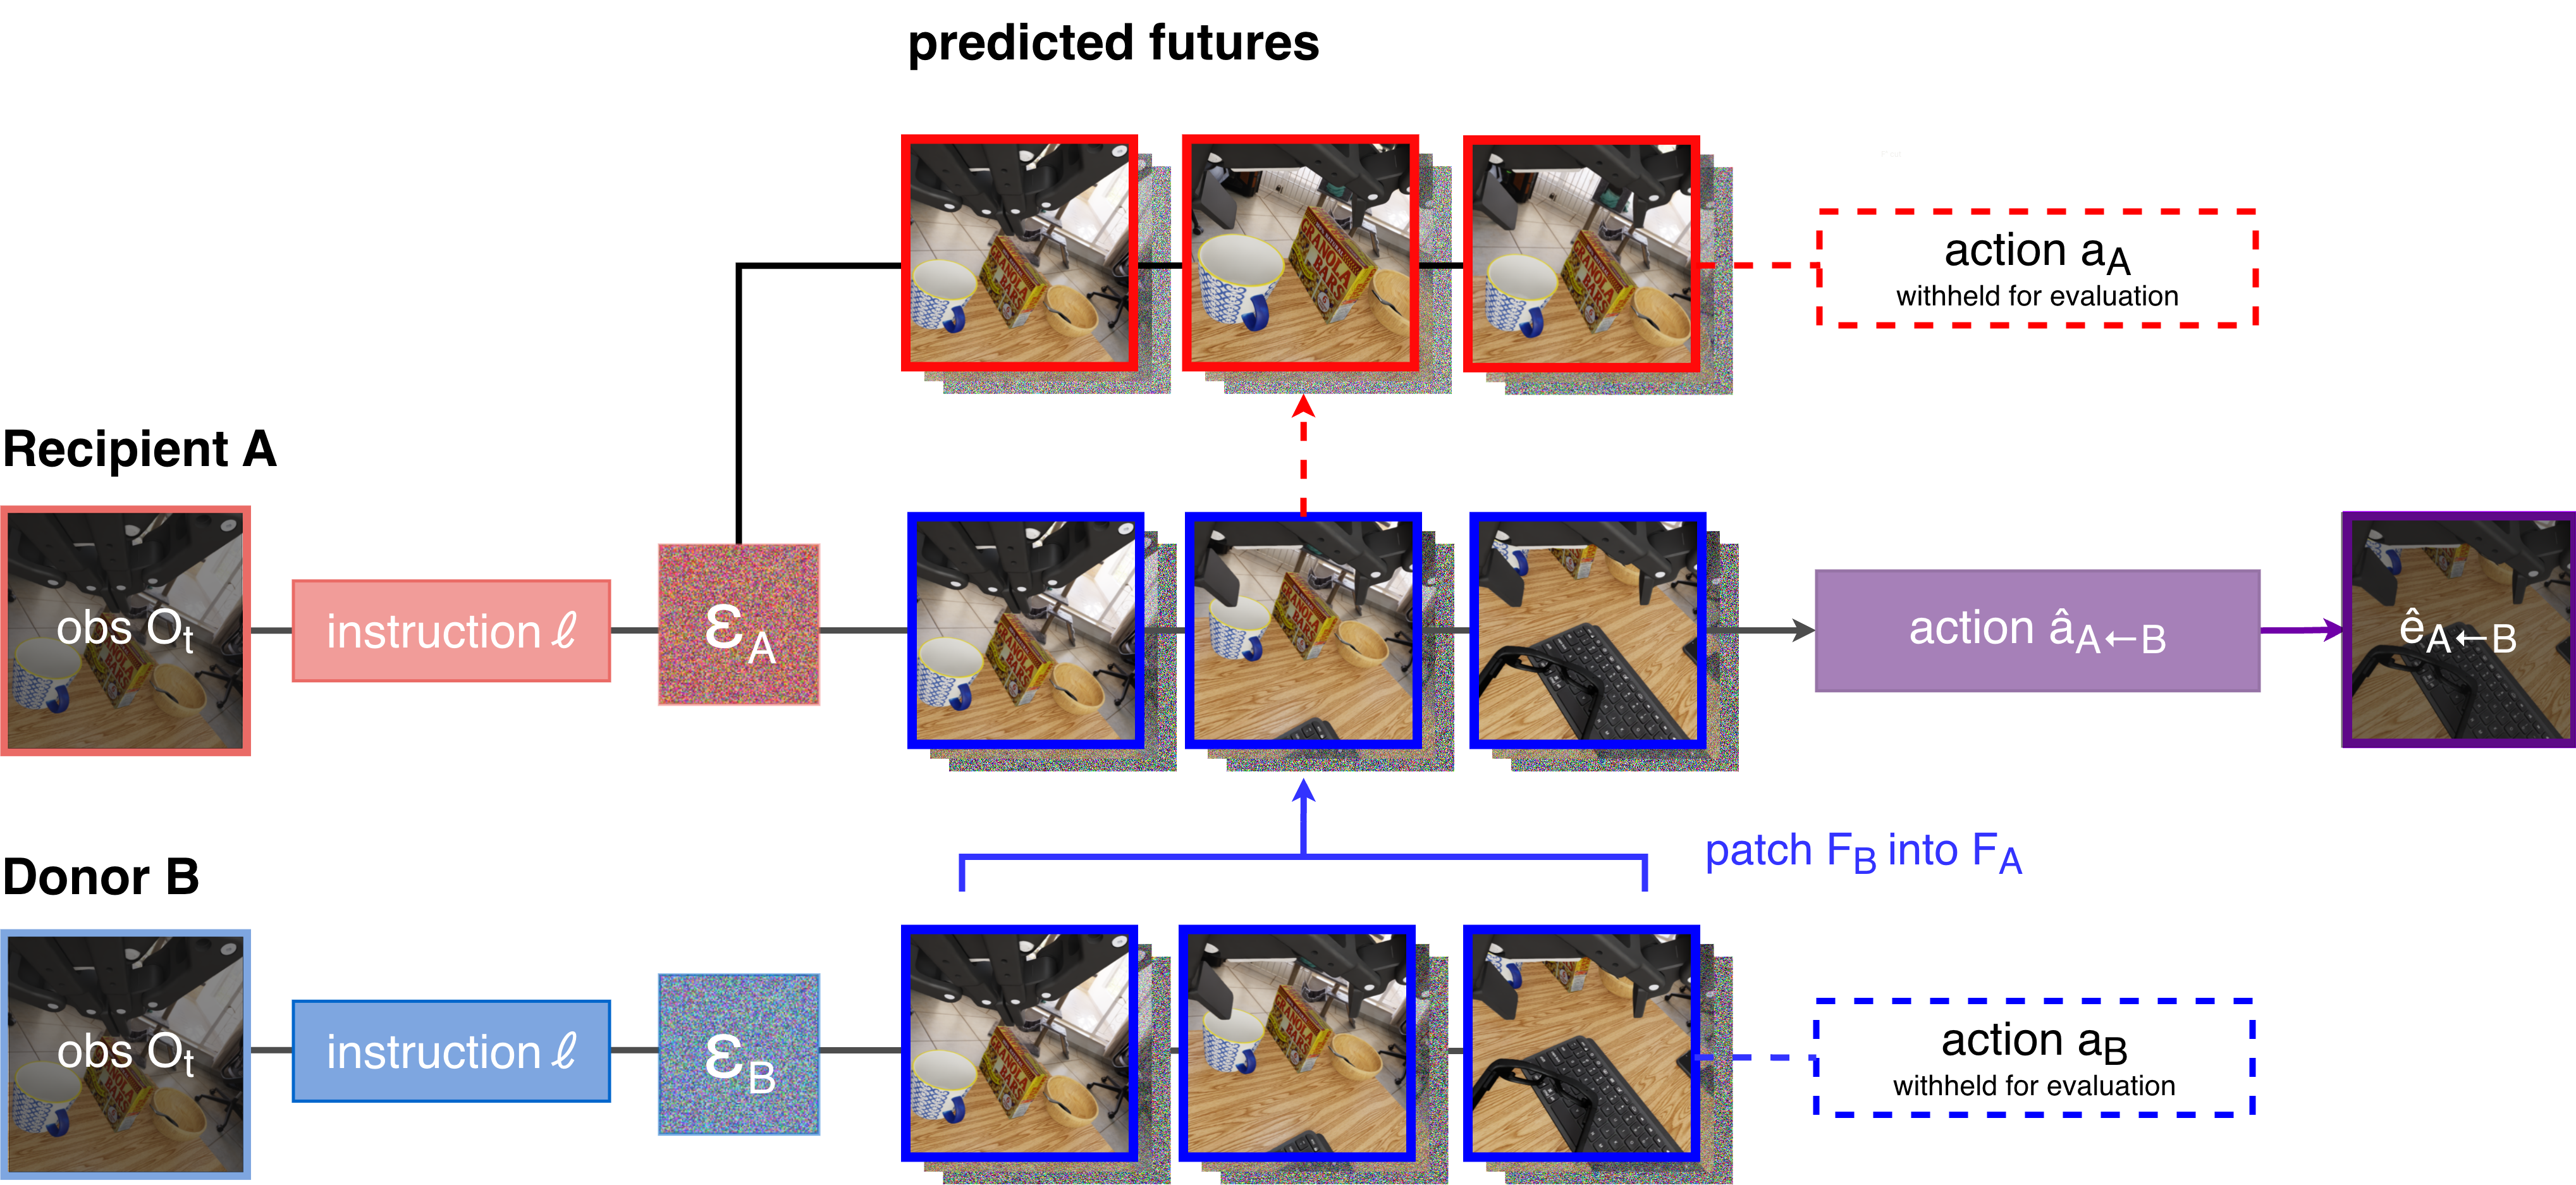
\includegraphics[width=0.96\textwidth]{figures/stage1_methodology.png}
  \caption{Future-content intervention. From native rollouts at the same state, Stage 1 inserts donor $B$'s future representation into recipient $A$ while holding the present and recipient action randomness fixed. We test whether the recomputed action and, where executed, endpoint move toward $B$; the donor action is withheld and used only for evaluation. The two-source schematic is repeated over complete four-source grids where supported.}
  \label{fig:stage1_method}
\end{figure*}

\subsection{Stage 1: Future-content intervention}
\label{sec:stage1}

Starting from state $S$, native rollouts produce future representations $F_j$ and paired actions $\mathbf a_j$ (Figure~\ref{fig:stage1_method}). We recompute recipient $i$ while replacing only its future representation with $F_j$. Observation, instruction, recipient action randomness, sampler, and action coordinates remain fixed. Model-specific insertion follows the released inference route: step-matched future clamping for Cosmos 3, matched donor latent-trajectory replay for DreamZero, and the future-derived cache for ordered video-first models. Cosmos Policy additionally encodes the endpoint of a native executed action, while Cosmos 3 tests predicted latents and executed videos. Appendix~\ref{app:future_replacement_impl} gives exact mechanics.

For action or endpoint $\mathbf x\in\{\mathbf a,\mathbf e\}$, normalized donor projection is
\begin{equation}
\pi_x(\hat{\mathbf x};R,D)=
\frac{(\hat{\mathbf x}-\mathbf x_R)^\top(\mathbf x_D-\mathbf x_R)}
{\lVert\mathbf x_D-\mathbf x_R\rVert_2^2}.
\label{eq:projection}
\end{equation}
The recipient is 0 and donor is 1; changes orthogonal to the donor direction receive little weight. We therefore pair projection with source retrieval: among four native candidate actions, the recomputed action must be nearest to the action paired with the installed source. Each state contributes 12 off-diagonal recipient--source cells, with 25\% chance under within-state label permutation. Every endpoint arm is executed after restoring the same state.

The matched four-source studies evaluate Cosmos 3 on 90 archival states from 30 episodes across six RoboLab tasks; FastWAM Optional-IDM on 120 states across all 40 LIBERO tasks; DreamZero on 30 deterministically selected states from distinct episodes and instructions in its released DROID training-data corpus; and LingBot-VA on 30 predetermined LIBERO-Long states across ten tasks \citep{nvidia2026cosmos3,nvidia2026cosmos3droid,yang2026robolab,yuan2026fastwam,ye2026dreamzero,li2026cauva,liu2023libero}. No source separation or intervention outcome enters cohort selection. Cosmos Policy retains its paired 30-state, ten-task study with physical replay \citep{kim2026cosmospolicy,nvidia2026cosmospolicylibero}. State is the independent unit; source directions and repeated draws are averaged within state, with model-specific frozen bootstrap intervals. Exact self/replay controls, model-specific no-op parity checks, and action-coordinate non-write audits test the implementations. Full designs appear in Appendix~\ref{app:settings}--\ref{app:stage1_stats}.

\begin{figure}[H]
  \centering
  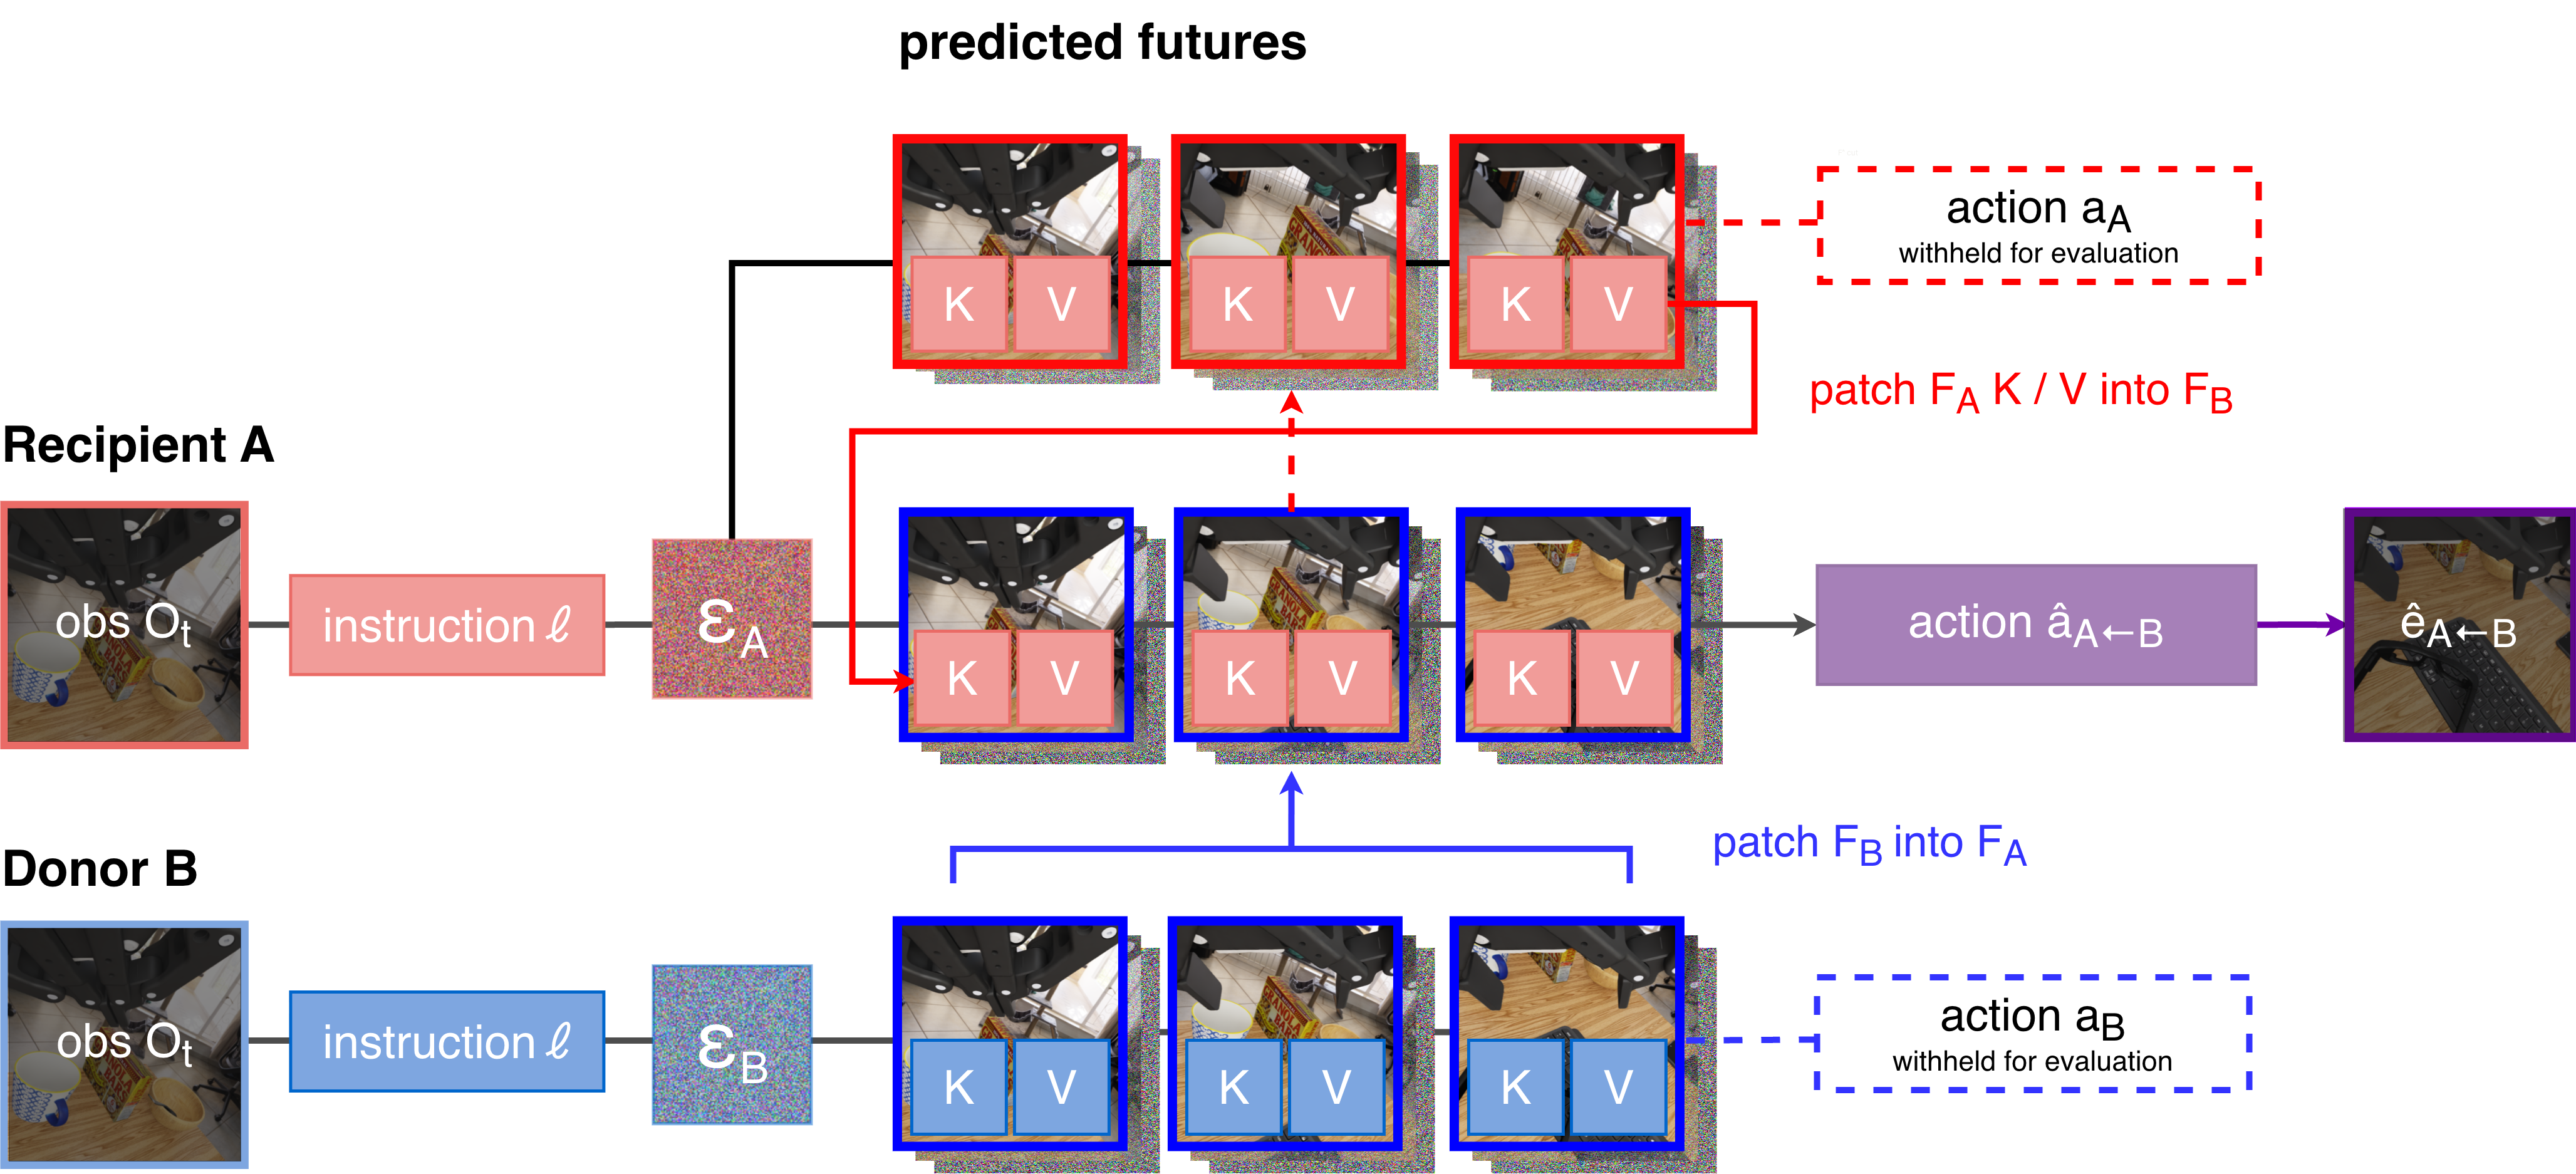
\includegraphics[width=0.96\textwidth]{figures/stage2_methodology.png}
  \caption{Stage-2 pathway intervention. We independently set visible-future identity and the source of predicted-future-position K/V read by action queries. The crossed cells test whether action follows the visible future or its K/V source.}
  \label{fig:stage2_method}
\end{figure}

\subsection{Stage 2: K/V pathway intervention}
\label{sec:stage2}

Stage 2 tests the direct future-to-action attention route in Cosmos 3. We record predicted-future-position K/V under recipient and donor futures, then independently cross visible future $F_R/F_D$ with K/V source $\kv_R/\kv_D$. This $2\times2$ design includes both suppression ($F_D,\kv_R$) and rescue ($F_R,\kv_D$), distinguishing routed source information from generic interface disruption. Cosmos Policy provides a separate prespecified key-removal test at block 27.

For Cosmos 3, K/V is recorded across all 36 layers and eight model forwards and replayed call by call. Only action-query attention outputs are recomputed; current-video and predicted-future query outputs remain native. Only future-position K/V are directly replaced; text, current-video, and action K/V are not overwritten. The interface was selected on excluded calibration tasks and frozen before population testing. Cache alignment, identity controls, and implementation details appear in Appendix~\ref{app:pathway_impl}.

\section{Results}
\label{sec:results}

\subsection{Future-source identity directionally controls action}
\label{sec:steering}

In the outcome-unfiltered Cosmos 3 cohort, the recomputed action identifies the installed future source in all 1,080 off-diagonal comparisons across 90 states (Table~\ref{tab:crossmodel}). Transplantation reduces distance to the source action by $0.763$ ($[0.733,0.792]$), with projection $0.966$ ($[0.956,0.974]$); the result holds in every decision phase and native-separation quartile. A separate selected-pair 22-state execution cohort links this action effect to behavior: predicted-future action steering is $0.992$, and executing the recomputed actions yields endpoint steering of $1.003$ ($[0.950,1.050]$; 22/22 states positive).

The same four-source test replicates across three released systems. FastWAM's explicit video-to-action route identifies the source in 1,439/1,440 off-diagonal cells, while its matched no-future route is exactly invariant to video seed. DreamZero's joint within-chunk denoising identifies 360/360 sources under matched per-step latent replay. LingBot-VA's ordered future-to-cache-to-action route identifies 269/360 ($0.747$; $[0.667,0.819]$), above the 25\% permutation null; this retrieval is primarily a later-chunk effect. Thus, simultaneous video/action denoising during action generation is not required. Pathwise dose tests are graded in both new systems: the three interior recipient-to-donor mixture levels are monotone in 30/30 DreamZero and 30/30 LingBot-VA states.

\begin{table}[H]
  \caption{Matched four-source predicted-action results. Each state contributes 12 off-diagonal source transplants. Intervals are model-specific frozen 95\% bootstrap CIs; models are not pooled.}
  \label{tab:crossmodel}
  \centering
  \scriptsize
  \setlength{\tabcolsep}{3.0pt}
  \begin{tabular}{@{}lrrrr@{}}
    \toprule
    System & States & Correct source & Distance reduction & Projection \\
    \midrule
    Cosmos 3 & 90 & \textbf{1080/1080} & 0.763 [0.733, 0.792] & 0.966 [0.956, 0.974] \\
    FastWAM & 120 & \textbf{1439/1440} & 0.683 [0.638, 0.738] & 0.869 [0.833, 0.912] \\
    DreamZero & 30 & \textbf{360/360} & 0.917 [0.897, 0.933] & 0.990 [0.984, 0.995] \\
    LingBot-VA & 30 & \textbf{269/360} & 0.473 [0.421, 0.524] & 0.675 [0.624, 0.723] \\
    \bottomrule
  \end{tabular}
\end{table}

Cosmos Policy supplies complementary physical evidence. At the first query of all ten LIBERO-Long tasks, paired-donor action projection is $0.499$ ($[0.336,0.679]$) and executed-endpoint projection is $0.552$ ($[0.387,0.728]$), both positive in 10/10 tasks. Its near-zero effect at separately sampled later states shows strong attenuation at later sampled states.

\subsection{Content profiles differ across architectures}
\label{sec:content}

Cosmos Policy's early-state effect is concentrated in future visual inputs, especially the wrist camera. Wrist-camera replacement produces action projection $0.435$ ($[0.284,0.605]$), primary-camera replacement $0.101$ ($[0.057,0.144]$), and future-proprioception replacement $0.001$ ($[-0.004,0.008]$). A separate rendered-video study finds an approximately zero object-state main effect on action and endpoint, while four exploratory natural-pair comparisons favor robot-motion futures. Together these results are most consistent with camera-visible prospective robot motion.

Cosmos 3 requires more than either isolated pixel factor. Across ten frozen states spanning all six tasks, a complete executed donor video strongly steers actions ($0.988$) and endpoints ($0.929$), but robot-pixel effects are $0.002$ and $0.010$ and object-pixel effects $0.006$ and approximately zero. Every isolated-factor interval lies inside the prespecified $[-0.10,0.10]$ equivalence region. This establishes isolated-factor insufficiency under the hybrid-mask design; the complete-video effect may depend on global context, tokenization or masking, distributed features, temporal robot--object coherence, or interactions among them (Appendix Figure~\ref{fig:cosmos3_factorization}).

\subsection{Future-token K/V redirects Cosmos 3 action}

The crossed $2\times2$ separates visible-future identity from future-token K/V source (Table~\ref{tab:kv_short}). With recipient visible future, changing recipient to donor K/V increases projection by $0.895$ ($[0.859,0.928]$); with donor visible future, the K/V effect is $0.885$ ($[0.845,0.921]$). Both crossed arms follow the K/V source in all 42 state-level comparisons. Donor K/V therefore rescues donor-directed action under a recipient visible future, while recipient K/V suppresses it under a donor future. The latter retains projection $0.119$ ($[0.078,0.162]$), so the route is major but incomplete. In the separate 22-state execution cohort, recipient-K/V restoration reduces endpoint steering by $0.851$ ($[0.766,0.922]$; 22/22 positive).

\begin{table}[t]
  \centering
  \caption{Cosmos 3 crossed future$\times$K/V intervention across 21 states. Entries are donor-axis action projection [95\% task$\rightarrow$state hierarchical-bootstrap CI].}
  \label{tab:kv_short}
  \scriptsize
  \setlength{\tabcolsep}{6pt}
  \begin{tabular}{@{}llc@{}}
    \toprule
    Visible future & Future-token K/V & Projection [95\% CI] \\
    \midrule
    Recipient & Recipient & $-0.011$ [$-0.022$, 0.000] \\
    Donor & Recipient & 0.119 [0.078, 0.162] \\
    Recipient & Donor & 0.884 [0.848, 0.919] \\
    Donor & Donor & 1.004 [0.988, 1.025] \\
    \bottomrule
  \end{tabular}
\end{table}

\section{Discussion and Limitations}

Controlled interventions turn an ambiguous co-generated output into testable claims about what controls action and how that effect is transmitted. Source-specific steering recurs in Cosmos 3 and DreamZero's joint within-chunk computations and in FastWAM and LingBot-VA's ordered video-first routes. LingBot-VA therefore rules out simultaneous video/action denoising during the action stage as a necessary explanation. Cosmos Policy connects steering to physical execution and shows that its early-state effect is concentrated in visual future targets. The Cosmos 3 factorial then shows that future-token K/V can suppress, rescue, and redirect the donor-axis action shift.

These results establish counterfactual control under future transplantation, not planning among alternatives. Planning would additionally require comparing predicted consequences using a goal or value and selecting among them. Our interventions instead isolate a prior question: whether changing a future representation redirects action toward the action associated with that source.

\paragraph{Limitations.}
The matched cross-model grids measure predicted action chunks; physical evidence comes from the Cosmos cohorts and remains one-chunk rather than closed-loop success. The archival Cosmos 3 grid uses lossy reconstructed inputs, DreamZero's analysis-held-out states come from its released training-data domain, and the evaluated LingBot-VA checkpoint was post-trained on the tested LIBERO-Long tasks. LingBot-VA source retrieval is primarily a later-chunk effect. External-model source hashes establish distinct native representations but do not by themselves label semantic differences between decoded videos. Pixel masks test localized factors, and K/V replacement isolates a specified interface rather than the complete circuit.

\paragraph{Responsible use.}
These methods could improve auditing by distinguishing visually plausible predictions from representations that actually control behavior. They could also redirect robot actions or encourage false confidence on narrow state distributions. Before physical deployment, mitigations should include broader coverage, independent replication, physical safety constraints, human oversight, and monitoring beyond the intervention metric.

\section{Conclusion}

Across four matched source-identification grids and complementary Cosmos execution studies, native future representations directionally control predicted actions under transplantation. Cosmos 3 future$\times$K/V interventions identify a major internal route that carries this source-specific effect.
